\section{Application Machine Learning}

In this section we will discuss the application of Gradient Flow
in Machine Learning. We first explain what Machine Learning
is, the connection to the theory of gradient flow
and then finish with an example and numerical experiment.
This section is based almost entirely on the lecture
notes of the course "Advancced Topics in Machine Learning"
from the University of Bern \cite{uniBernLecNotes}.

\subsection{Gradient Flow in Training of Neural Networks}
In many applications of machine learning, we are dealing
with an unknown probability distribution $ \mu $ on
$ \rX\times \rY$ with a set of features $ \rX $
and a set of targets $ \rY $. Given some 
loss function $ L:\rY\times \rY\rightarrow\RR $
we want to solve the following optimization problem,
referred to as Bayes Risk,
\begin{align}\label{equation:Bayes Risk}
	\minimize_{f:\rX\ra\rY}
	\qquad &\qquad
	\int_{\rX\times \rY} L(f(x),y)\,d\mu(x,y).
	\tag{BR}
\end{align}
In practice the only information we
have of the distribution $ \mu $
is a finite dataset $ \daSet\subseteq\rX\times\rY $
drawn independently under the distribution $ \mu $. 
We approximate $ \mu $ by the empirical risk as a 
probability measure $ \emMe $ on $ \rX\times\rY $ defined by
\begin{align*}
	\emMe:=\frac{1}{\vert \daSet\vert}\sum_{(x,y)\in\daSet}\delta_{(x,y)}.
\end{align*}
With this probability measure our optimization problem becomes
\begin{align}\label{equation:emp Bayes Risk}
	\minimize_{f:\rX\ra\rY}
	\qquad &\qquad
	\int_{\rX\times \rY} L(f(x),y)\,d\emMe(x,y).
	\tag{eBR}
\end{align}
In many applications we must approximate the optimal solution 
by functions that are parametrisable by some weight.
A highly versatile family of such functions are called
neural networks. The set of all neural networks $ N $ is given inductively by
\begin{enumerate}[label=(\roman*)]
	\item For any map $ f:\RR^n\times \RR^k\ra \RR^m $
	and any weight $ \theta\in \RR^k $,
	the set of all neural networks $ N $ contains
	the function $ \RR^n\ra\RR^m;\,x\mapsto f(x;\,\theta):=f(x,\theta) $.
	We say $ f(\bullet;\,\theta) $ is a layer with weight $ \theta $ and
	$ f(\bullet;\,\theta)_j $ is a node of the layer for $ 1\leq j\leq m $.
	\item Let $ g(\bullet;\,\theta):\RR^n\rightarrow \RR^m $ be 
	some neural network in $ N $
	weighted by $ \theta\in\RR^k $
	and $ h:\RR^m\ra \RR^r $ be some layer in $ N $ weighted by 
	$ \pi \in \RR^s$. Then the
	composition $ f(\bullet;\theta,\pi):=h(g(\bullet;\theta);\pi) $ 
	is another neural 
	network in $ N $ weighted by $ (\theta,\pi) $. For the particular
	neural network $ f(\bullet;\theta,\pi) $, we call
	$ h $ the output layer. Similarly we call the first layer
	in the composition of a neural network the input layer.
\end{enumerate}

%From https://texample.net/tikz/examples/neural-network/
\begin{figure}[t]
	\centering
	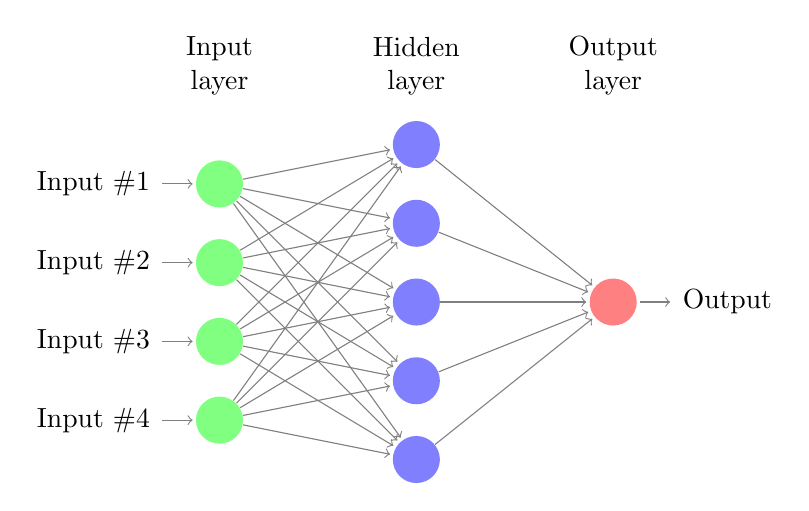
\begin{tikzpicture}[shorten >=1pt,->,draw=black!50, node distance=\layersep]
		\def\layersep{2.5cm}
		
		\tikzstyle{every pin edge}=[<-,shorten <=1pt]
		\tikzstyle{neuron}=[circle,fill=black!25,minimum size=17pt,inner sep=0pt]
		\tikzstyle{input neuron}=[neuron, fill=green!50];
		\tikzstyle{output neuron}=[neuron, fill=red!50];
		\tikzstyle{hidden neuron}=[neuron, fill=blue!50];
		\tikzstyle{annot} = [text width=4em, text centered]
		
		% Draw the input layer nodes
		\foreach \name / \y in {1,...,4}
		% This is the same as writing \foreach \name / \y in {1/1,2/2,3/3,4/4}
		\node[input neuron, pin=left:Input \#\y] (I-\name) at (0,-\y) {};
		
		% Draw the hidden layer nodes
		\foreach \name / \y in {1,...,5}
		\path[yshift=0.5cm]
		node[hidden neuron] (H-\name) at (\layersep,-\y cm) {};
		
		% Draw the output layer node
		\node[output neuron,pin={[pin edge={->}]right:Output}, right of=H-3] (O) {};
		
		% Connect every node in the input layer with every node in the
		% hidden layer.
		\foreach \source in {1,...,4}
		\foreach \dest in {1,...,5}
		\path (I-\source) edge (H-\dest);
		
		% Connect every node in the hidden layer with the output layer
		\foreach \source in {1,...,5}
		\path (H-\source) edge (O);
		
		% Annotate the layers
		\node[annot,above of=H-1, node distance=1cm] (hl) {Hidden layer};
		\node[annot,left of=hl] {Input layer};
		\node[annot,right of=hl] {Output layer};
	\end{tikzpicture}
	\caption{A common graphical representation of a neural network.}
	\label{figure:gr rep nn}
\end{figure}

A neural network is commonly graphically represented as seen in
figure \ref{figure:gr rep nn}. The reason the family
of functions are called neural networks is that
the graph resembles a biological neural network.\medskip

In practice a neural network is an alternating sequence between 
affine layers of the form $ f(x;A,b)=Ax+b $ for a weight 
$ (A,b)\in\RR^{m\times n}\times \RR^m $
and some choice of non-linear layers $ h:\RR^n\rightarrow\RR^m $,
such as the sigmoid function 
$ s:\RR\ra \RR;\,x\mapsto (1+\exp(-x))^{-1} $ or
the rectified linear unit function
$ \mathrm{ReLu}:\RR\ra \RR;\,x\mapsto\max\{0,x\} $
applied entry-wise to the input. These non-linear mappings
are called activation functions.\medskip

The approximation of the ideal function with some neural network
is prone to generalization errors. To combat this, we often add
a regularization function $ R:\RR^n\times \RR^m\ra \RR $. 
As an example we may demand that the 
output data to be sparse. In this case we could choose
$ R(x,\theta)=\abs{x_1}+\ldots+\abs{x_n} $ for 
$ (x,\theta)\in\RR^{n}\times\RR^m $. Our minimization
problem thus becomes 
\begin{align*}\label{equation:reg emp Bayes Risk}
	\minimize_{\theta\in \RR^k}
	\qquad &\qquad
	\int_{\rX\times \rY} L(f(x;\theta),y)+R(f(x;\theta),\theta)\,d\emMe(x,y).
	\tag{Reg-eBR}
\end{align*}

We extract two function definitions 
\begin{align*}
	\vp(\theta):=\int_{\rX\times \rY} L(f(x;\theta),y)\,d\emMe(x,y)
	\quad\text{ and }\quad
	\psi(\theta):=\int_{\rX\times \rY} R(f(x;\theta),\theta)\,d\emMe(x,y).
\end{align*}

and restate state our minimization problem as the general problem
\begin{align*}
	\minimize_{\theta\in \RR^k}
	\qquad &\qquad
	\vp(\theta)+\psi(\theta).
\end{align*}

Usually the only assumption we place on $ \vp $ is that
it is Lipschitz continuous. However for many applications 
we may assume that $ \vp $ is a proper convex
differentiable function and that $ \psi $ is a proper convex function
(cf. \cite[Section 3.1]{signoretto2014learning}).
In this case we know from 
% TODO find source
\cite{rockafellar2015convex} 
that $ \theta^{\ast}\in\RR^k $
is an optimal solution to the minimization problem
if and only if
\begin{align*}
	0\in \prt f(\theta^{\ast})+\prt g(\theta^{\ast}).
\end{align*} 
Provided that both $ \vp $ and $ \psi $ are l.s.c,
the operator $ A:=\prt f+\prt g $
is maximally monotone by 
corollary \ref{corollary:sub diff of pr lsc func is max mon op}.
We find the optimal solution by solving the evolution
equation \ref{equation:hom GSD}
with operator $ A $ and any
initial value $ \theta_0\in \RR^k $. In particular
we solve
\begin{align*}
	\begin{cases}
		\partial_t \theta+A\theta \ni 0 & \text{ on }[0,\plus\infty),\\
		\theta=\theta_0 & \text{ on }\{0\}.
	\end{cases}
\end{align*}

In practice it is far more efficient and suffices to approximate the solution
by the discrete gradient descent algorithm,
instead of solving the actual evolution
equation. The generalized discrete gradient
descent method is given by the forward Euler method  
\begin{align}\label{equation:disc grad desc meth}
	\begin{cases}
		\theta_t-(\idm_{\RR^k}-\alpha A)\theta_{t-1} \ni 0 & \text{ on }\NN,\\
		\theta_t=\theta_0 & \text{ on }\{0\}.
	\end{cases}
	\tag{gDGM}
\end{align}
for some user defined step size $ \alpha>0 $.
The theory of gradient flows applies
to non-convex functions as-well, however
fewer properties are known and the
asymptotic limit may change depending
on the initial value.

\subsection{Example Ridge Regression}
The paper \cite[Section 3.2]{signoretto2014learning} from M. Signoretto et al
mentions two examples of how the gradient descent method
can be applied, where the minimization function
is convex. Namely Ridge Regression \cite{hoerl1970ridge}
and Group Lasso \cite{jacob2009group}. We will present
an example of Ridge Regression as it is very simple,
a smooth and convex problem,
and it highlights important aspects of machine learning.
\smallskip

Ridge Regression is a method for solving the standard model for 
linear regression. Suppose that there
exists some unknown affine linear transformation
$ h:\RR^k\ra \RR $. We are given a finite dataset
$ (X_1,Y_1),\ldots,(X_n,Y_n)\in\RR^{k}\times \RR $
such that $ Y_i=h(X_i)+\varepsilon_i $ for
all $ 1\leq i\leq n $, where the variables
$ \varepsilon_1,\ldots,\varepsilon_n $
are unknown and are chosen i.i.d from some  
probability distribution.\smallskip

Naturally we will try to approximate the
linear functional $ h $ with a single
layer affine neural network defined by
$ f(x;a,b):=a^t x+b $ for any 
$ x,a\in\RR^k $ and $ b\in\RR $.\smallskip

We define our loss function $ L $ as the squared error 
\begin{align*}
	L(x,y):=\frac{1}{2}(x-y)^2
	\qquad\forall x,y\in\RR.
\end{align*}

We want to control the growth of
the weights $ a,b $ with some
user defined
parameter $ \lambda>0 $ by the 
regularization function
\begin{align*}
	R(a,b):=\frac{\lambda}{2}(a^ta+b^2)
	\qquad\forall (a,b)\in\RR^k\times\RR.
\end{align*}

Our problem statement \ref{equation:reg emp Bayes Risk}
thus becomes
\begin{align*}
	\minimize_{(a,b)\in \RR^n\times\RR}
	\qquad &\qquad
	\frac{\lambda}{2}(a^ta+b^2)+
	\frac{1}{2n}\sum_{i=1}^n (Y_i-f(X_i;a,b))^2.
\end{align*}

We use matrix notation to simplify the above expression.
To that end define $ X\in\RR^{n\times k} $ by $ X:=(X_1,\ldots, X_n)^t $,
define $ Y\in\RR^n $ by $ Y:=(Y_1,\ldots,Y_n) $ and define
the vector the constant one vector $ e:=(1,\ldots,1)\in\RR^n $. We compute
\begin{align*}
	\frac{1}{2n}\sum_{i=1}^n (Y_i-f(X_i;a,b))^2
	&=\frac{1}{2n}(Y-Xa-be)^t(Y-Xa-be)\\
	&=\frac{1}{2n}
	\begin{pmatrix}
		a \\ b
	\end{pmatrix}^t
	\begin{pmatrix}
		X^t X & 0\\
		0 & 1
	\end{pmatrix}
	\begin{pmatrix}
		a \\ b
	\end{pmatrix}
	-\frac{1}{n}
		Y^t 
	\begin{pmatrix}
		X & e
	\end{pmatrix}
	\begin{pmatrix}
		a \\ b
	\end{pmatrix}
	+\frac{1}{2n}Y^tY.
\end{align*}
Then the \ref{equation:reg emp Bayes Risk} equation can be simplified to

\begin{align*}
	\minimize_{(a,b)\in \RR^n\times\RR}
	\quad &\quad
	\begin{pmatrix}
		a \\ b
	\end{pmatrix}^t
	\left(
	\frac{\lambda}{2}
	\idm_{\RR^{k+1}}
	+
	\frac{1}{2n}
	\begin{pmatrix}
		X^t X & 0\\
		0 & 1
	\end{pmatrix}
	\right)
	\begin{pmatrix}
		a \\ b
	\end{pmatrix}
	-\frac{1}{n}
		Y^t
	\begin{pmatrix}
		X & e
	\end{pmatrix}
	\begin{pmatrix}
		a \\ b
	\end{pmatrix}
	+\frac{1}{2n}Y^tY.
\end{align*}
We see that we must minimize a quadratic polynomial, which happens
to be a proper convex smooth problem. Thus our theory is applicable.\smallskip

To deduce the discrete gradient descent method
we must simply compute the derivative of $ a $
and $ b $
\begin{align*}
	\Delta(a,b):=&\prt_{(a,b)}
	\begin{pmatrix}
		a \\ b
	\end{pmatrix}^t
	\left(
	\frac{\lambda}{2}
	\idm_{\RR^{k+1}}
	+
	\frac{1}{2n}
	\begin{pmatrix}
		X^t X & 0\\
		0 & 1
	\end{pmatrix}
	\right)
	\begin{pmatrix}
		a \\ b
	\end{pmatrix}
	-\frac{1}{n}
		Y^t
	\begin{pmatrix}
		X & e
	\end{pmatrix}
	\begin{pmatrix}
		a \\ b
	\end{pmatrix}
	+\frac{1}{2n}Y^tY\\
	&\qquad=\left(
	\lambda\idm_{\RR^{k+1}}
	+
	\frac{1}{n}
	\begin{pmatrix}
		X^t X & 0\\
		0 & 1
	\end{pmatrix}
	\right)
	\begin{pmatrix}
		a \\ b
	\end{pmatrix}
	-\frac{1}{n}
	\begin{pmatrix}
		X^t \\ e^t
	\end{pmatrix}
	Y.
\end{align*}

The discrete gradient descent method is therefore given by
\begin{align*}
	\begin{cases}
		(a_t,b_t)-(a_{t-1},b_{t-1})
		+\alpha \Delta(a_{t-1},b_{t-1}) = 0 & \text{ on }\NN,\\
		(a_t,b_t)=(a_0,b_0) & \text{ on }\{0\}.
	\end{cases}
\end{align*}

\subsubsection{Numerical Experiment}
We end the paper by presenting a concrete example of ridge
regression\footnote{all of the code that
was used in this experimenter is found in the following
GitHub repository}. Given some dimension $ k $, some fixed $ a_{\mathrm{real}}\in\RR^k $
and $ b_{\mathrm{real}}\in\RR $, we will use the discrete gradient descent method to
approximate the linear functional
$ h_{\mathrm{real}}(x):=a_{\mathrm{real}}^t x +b_{\mathrm{real}}$.
We choose $ n $ points $ X_1,\ldots,X_n $ independently under
a uniform distribution from an open subset $ \Omega\subseteq\RR^k $.
For some user defined $ \sigma>0 $, we draw $ n $
values $ \varepsilon_1,\ldots,\varepsilon_n $ independently 
from the normal distribution
$ \mathcal{N}(0,\sigma^2) $ and define $ Y_i:=h_{\mathrm{real}}(X_i)+\varepsilon_i $
for $ 1\leq i\leq n $. We choose the initial weights $ (a_0,b_0) $ uniformly
randomly from an open set $ \Theta\subseteq\RR^k\times\RR $.\medskip

This numerical experiment is conducted using MatLab
and the standard random number generator provided by MatLab.
The source code is available at this public
\href{https://github.com/JethroWarnettMath/Semester-Project-Gradient-Flow-HS2021}
{GitHub} repository.\medskip

For our experiment we set $ k=2 $, 
$a_{\mathrm{real}}=(1,-1)$, $ b_{\mathrm{real}}=2 $,
$ \Omega=[-10,10]^2 $ and $ \Theta=[-10,10]^3 $. 
With these parameters we let the discrete gradient descent
algorithm run for a $ 1000 $ iterations. We repeat the
experiment $ 10 $ times and plot the results in the
following figures:\smallskip 

In figure 3 %\ref{fig:exampleA} 
we show how the parameter $ a_t $ evolves depending
on its initial weight. We
see that for each starting value the graphs 
more or less converge in a straight line to 
the value $ a_{\mathrm{real}} $. \smallskip

In figure 4 we
present how the parameter $ b_t $ changes depending
on its initial weight. Again we
see that for each starting value the graphs 
converge to the value $ b_{\mathrm{real}} $. \smallskip

Finally in figure 5 we
present how the parameter $ a_b $ develops depending
on its initial weight. For each starting value the graphs 
decay linearly to $ 0 $.

\begin{figure}[H]
	\centering
	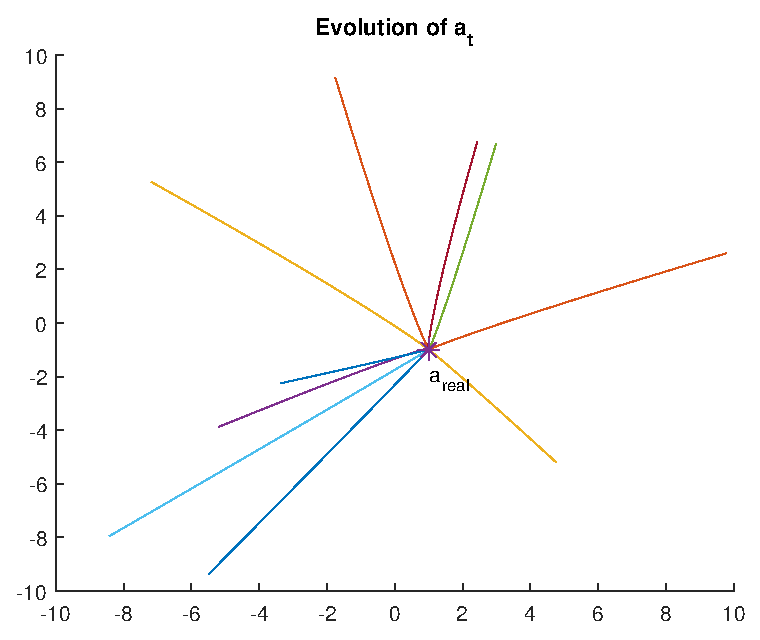
\includegraphics[width=0.5\linewidth]{EvolutionA}
	\caption{The evolution of $ a_t $ in the
	discrete gradient descent method for different
	initial values.}\label{fig:exampleA}
\end{figure}

\begin{figure}[H]
	\centering
	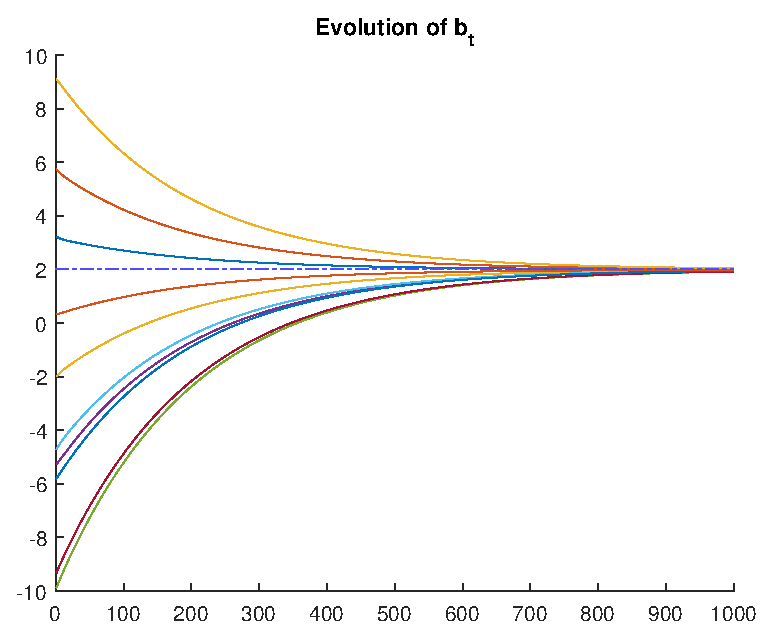
\includegraphics[width=0.5\linewidth]{EvolutionB}
	\caption{The evolution of $ b_t $ in the
		discrete gradient descent method for different
		initial values.}\label{fig:exampleB}
\end{figure}

\begin{figure}[H]
	\centering
	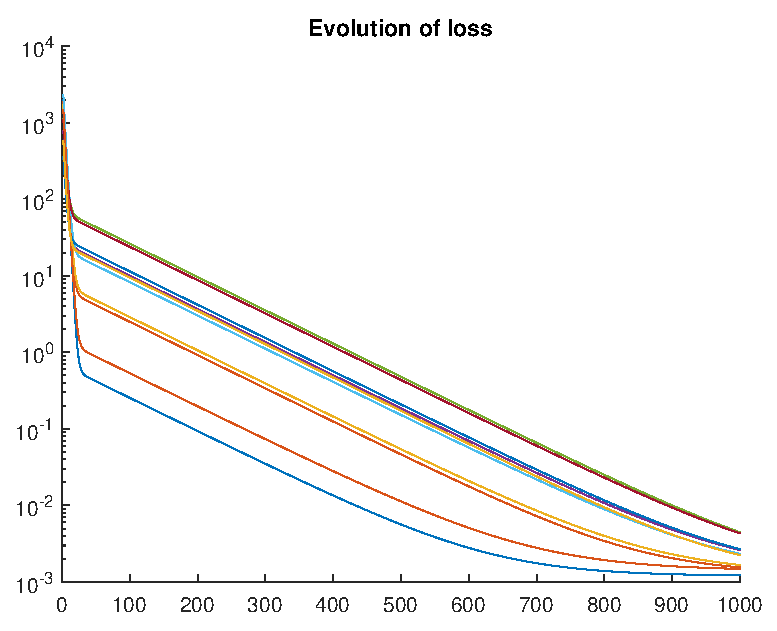
\includegraphics[width=0.5\linewidth]{EvolutionLoss}
	\caption{The evolution of the loss function in the
		discrete gradient descent method for different
		initial values. Note that the scale is logarithmic
		in the y axis.}\label{fig:exampleLoss}
\end{figure}